
\subsection{Group 2 - Blockchain Knowledge and Opinions}

\subsection*{1 - General Blockchain Knowledge.}
 %GRAFICO BLOCKCHAIN KNOWLEDGE
 \begin{figure}[h]
\centering
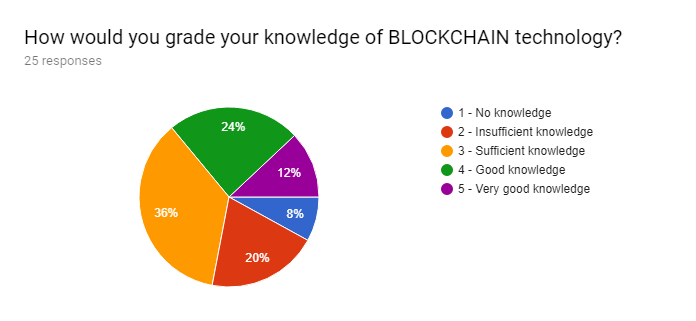
\includegraphics[scale=0.65]{media/blockchain_knowledge.png}
\caption["Blockchain knowledge."]{Blockchain knowledge.}
\label{fig:blockchain_knowledge}
\end{figure}
 
 
\subsection*{2 - Rate the affirmations about the use of cryptocurrencies in the blockchain.}

\begin{figure}[h]
\centering
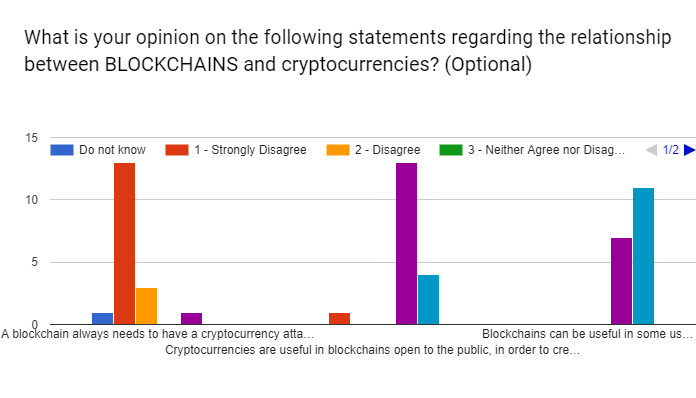
\includegraphics[scale=0.60]{media/blockchain_crypto_opinions.png}
\caption[Rate the affirmations about the use of cryptocurrencies in the blockchain]{Rate the affirmations about the use of cryptocurrencies in the blockchain}
\label{fig:blockchain_crypto_opinions}
\end{figure}

\todo{fcorreia: a legenda da figura está a ser cortada}

%GRAFICOS DE CADA 1 DAS 3 AFIRMAÇÕES DE CRYPTOCURRENCIES
\textbf{Affirmations: }
\begin{enumerate}
\item A blockchain always needs to have a cryptocurrency attached in order to work well.
\item Cryptocurrencies are useful in blockchains open to the public, in order to create incentives for good behavior, but not always necessary in private chains.
\item Blockchains can be useful in some uses cases, independently of whether they hold a cryptocurrency or not.
\end{enumerate}


\todo{fcorreia: eu tiraria os prefixos "Affirmation 123" e deixava diretamente a pergunta em cada celula. acho que basta para se perceber. no caption podes clarificar que a tabela se refere às perguntas na categoria "Blockchain Knowledge and Opinions"}

\todo{fcorreia: está um pouco grande esta tabela. dá para reduzir ao tamanho de letra dos titulos das colunas e das perguntas?}

%%%%%% TABLE START %%%%%%%%%%%%%%
% Please add the following required packages to your document preamble:
% \usepackage[normalem]{ulem}
% \useunder{\uline}{\ul}{}
\begin{table}[ht]
\centering
\begin{tabular}{l|c|c|c|c|c|c|}
\cline{2-7}
                                                                                                                                                                       & \multicolumn{1}{l|}{Mode} & \multicolumn{1}{l|}{Median} & \multicolumn{1}{l|}{Mean} & \multicolumn{1}{l|}{\begin{tabular}[c]{@{}l@{}}Standard\\  Deviation\end{tabular}} & \multicolumn{1}{l|}{Range} & \multicolumn{1}{l|}{Skewness} \\ \hline
\multicolumn{1}{|l|}{\begin{tabular}[c]{@{}l@{}}Affirmation 1 - Blockchain needs\\ cryptocurrencies to work well\end{tabular}}                                          & 1                         & 1                           & 1,3529                    & 0,7859                                                                             & 3                          & 2,7418                        \\ \hline
\multicolumn{1}{|l|}{\begin{tabular}[c]{@{}l@{}}Affirmation 2 - Cryptocurrencies\\ are only useful as incentives in\\ public blockchains\end{tabular}}                  & 4                         & 4                           & 4,0556                    & 0,8726                                                                             & 4                          & -2,5059                       \\ \hline
\multicolumn{1}{|l|}{\begin{tabular}[c]{@{}l@{}}Affirmation 3 - Blockchains can\\ be useful in some cases, regardless\\ of having or not cryptocurrencies\end{tabular}} & 5                         & 5                           & 4,6111                    & 0,5016                                                                             & 1                          & -0,4984                       \\ \hline
\end{tabular}
\caption{My caption}
\label{my-label}
\end{table}

%%%%%%%%%%% TABLE END %%%%%%%%%%%%%%%%%%%%%%%%%%%

TEST TEST: TALK ABOUT THE TABLE AND AFFIRMATIONS HERE

\subsection*{3 - Blockchain adoption challenges - maybe this one isnt that important to show}
% MAYBE TAKE THIS ONE OUT - NOT THAT IMPORTANT
